% Figure from MATH 591 notes, section 12. Compile with the notes preamble.
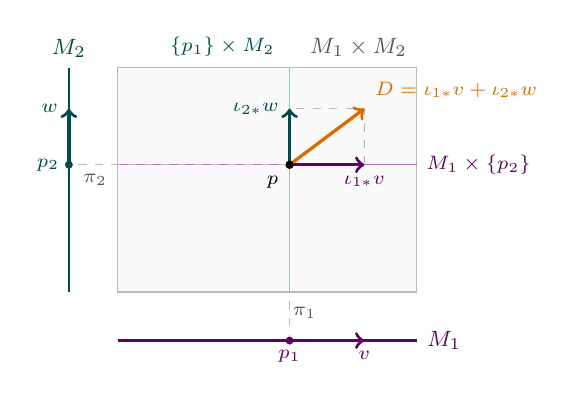
\begin{tikzpicture}[scale=0.95]
\fill[gray!5] (0,0) rectangle (4,3); \draw[gray!55] (0,0) rectangle (4,3); \node[font=\footnotesize, gray!70!black, anchor=south east] at (4,3.02) {$M_1 \times M_2$};
\draw[violet!75!black, thick] (0,-0.65) -- (4,-0.65) node[right, font=\footnotesize] {$M_1$};
\draw[teal!60!black, thick] (-0.65,0) -- (-0.65,3) node[above, font=\footnotesize] {$M_2$};
\draw[violet!55] (0,1.70) -- (4,1.70) node[right, font=\scriptsize, text=violet!75!black] {$M_1 \times \{p_2\}$};
\draw[teal!45] (2.30,0) -- (2.30,3);  \node[font=\scriptsize, text=teal!60!black, anchor=south] at (1.40,3.02) {$\{p_1\} \times M_2$};
\draw[gray!55, dashed] (3.30,1.70) -- (3.30,2.45) -- (2.30,2.45);
\draw[->, very thick, violet!75!black] (2.30,1.70) -- (3.30,1.70) node[below, font=\scriptsize] {$\iota_{1*}v$};
\draw[->, very thick, teal!60!black] (2.30,1.70) -- (2.30,2.45) node[left, font=\scriptsize] {$\iota_{2*}w$};
\draw[->, very thick, orange!85!black] (2.30,1.70) -- (3.30,2.45) node[above right, font=\scriptsize] {$D = \iota_{1*}v + \iota_{2*}w$};
\fill (2.30,1.70) circle (1.6pt); \node[font=\scriptsize, anchor=north east] at (2.28,1.68) {$p$};
\draw[gray!55, dashed] (2.30,1.65) -- (2.30,-0.65); \draw[gray!55, dashed] (2.25,1.70) -- (-0.65,1.70);
\fill[violet!75!black] (2.30,-0.65) circle (1.5pt) node[below, font=\scriptsize] {$p_1$}; \draw[->, very thick, violet!75!black] (2.30,-0.65) -- (3.30,-0.65) node[below, font=\scriptsize] {$v$};
\fill[teal!60!black] (-0.65,1.70) circle (1.5pt) node[left, font=\scriptsize] {$p_2$}; \draw[->, very thick, teal!60!black] (-0.65,1.70) -- (-0.65,2.45) node[left, font=\scriptsize] {$w$};
\node[font=\scriptsize, gray!70!black] at (2.50,-0.28) {$\pi_1$}; \node[font=\scriptsize, gray!70!black] at (-0.3,1.50) {$\pi_2$};
\end{tikzpicture}
